\section{Factorial Closure and Response-Class Audits}
\label{sec:experiments}

The evidence has two deliberately different layers.  A controlled real-data
experiment closes the complete chain from hidden strong convexity through
Schur curvature, M\"obius effects, experimental design, inference,
falsification, and finite-response tracking.  Neural-network trace audits then
test whether the declared response classes remain informative in nonconvex
training.  Only the first layer is a direct validation of the
reduced-value interaction law.

\subsection{A real-data hidden optimization model}

We use the handwritten digits 3 and 8 from the scikit-learn digits data.  A
stratified split gives 249 training and 108 test examples.  After standardizing
the 64 pixels and adding an intercept, the hidden state is
$w\in\R^{65}$.  The base energy is ridge logistic regression,
\[
E_0(w)=\frac1N\sum_{n=1}^N
\log(1+e^{-y_nx_n^\top w})+\frac{\lambda}{2}\norm w^2,
\qquad \lambda=0.15.
\]
Three continuous interventions $u\in[0,1]^3$ emphasize the digit-3 examples,
the digit-8 examples, and a central-$2\times2$-occlusion robustness loss.  If
$\Delta_i$ is the corresponding mean logistic loss, the hidden energy and
declared response are
\begin{equation}
E(w,u)=E_0(w)+0.75\sum_{i=1}^3u_i\Delta_i(w),
\qquad
F(u)=\min_w E(w,u).
\label{eq:digits-hidden-energy}
\end{equation}
Every added loss is convex, so $E_{ww}\succeq0.15I$ on the whole intervention
cube and every configuration has a unique global minimizer.  The largest
terminal gradient infinity norm across the eight Boolean solves is
$3.09\times10^{-13}$.

\subsection{Curvature, Boolean effects, and continuous prediction}

Boolean effects are computed from eight independently optimized corner
responses.  Separately, order-24 Gauss--Legendre quadrature evaluates
$-g_i^\top H^{-1}g_j$ after resolving the hidden optimum at every quadrature
node.  Neither path uses the output of the other.

\begin{table}[t]
\centering
\caption{Independent Boolean and curvature-integral evaluations for the three
mechanism pairs in \cref{eq:digits-hidden-energy}.  Pair 1--2 emphasizes the
two classes; pairs 1--3 and 2--3 combine class information with occlusion
robustness.}
\label{tab:interaction-curvature-closure}
\small
% Generated by interaction_curvature_experiment.py
\begin{tabular}{lrrr}
\toprule
Pair & Boolean effect & Curvature integral & Abs. error \\
\midrule
1-2 & +0.000625 & +0.000625 & 8.36e-15 \\
1-3 & -0.007276 & -0.007276 & 4.21e-11 \\
2-3 & -0.014264 & -0.014264 & 3.16e-11 \\
\bottomrule
\end{tabular}

\end{table}

\begin{figure}[t]
\centering
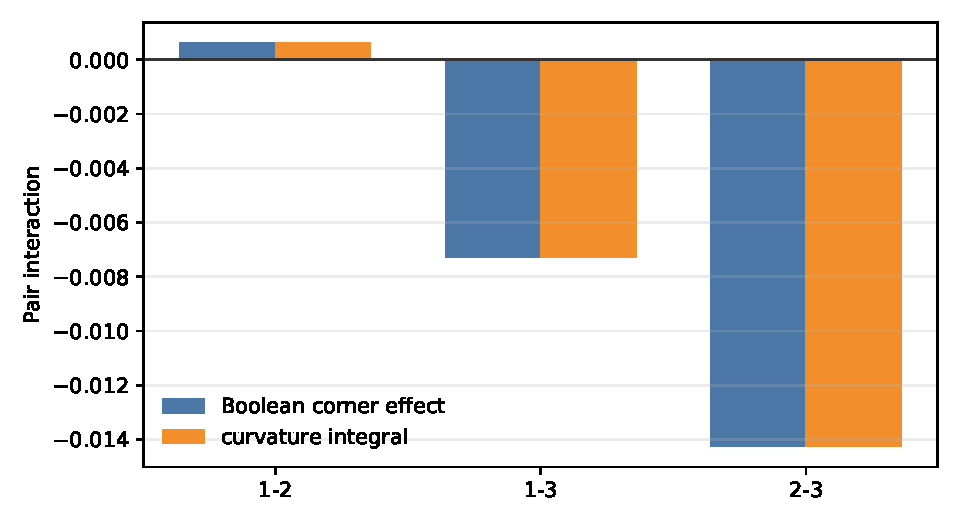
\includegraphics[width=0.72\linewidth]{figures/interaction_curvature_validation.pdf}
\caption{Boolean pair effects and independently integrated Schur curvature.
The largest absolute discrepancy is $4.21\times10^{-11}$.}
\label{fig:interaction-curvature-validation}
\end{figure}

Across the three pairs, the maximum Boolean identity error is
$4.21\times10^{-11}$.  We also reserve three non-Boolean intensity points per
pair, $(0.2,0.7)$, $(0.45,0.35)$, and $(0.8,0.55)$.  Direct joint optimization
and edge-response-plus-curvature reconstruction agree at all nine points with
maximum error $8.88\times10^{-13}$.  Repeating all Boolean solves and three
curvature integrals on eight independent stratified data splits gives 24
additional identities with maximum error $2.81\times10^{-8}$.  The small
class--class effect changes sign across splits, whereas both
class--occlusion effects remain negative.

\subsection{Information design and Gaussian confirmation}

We declare the order-two support
\[
\Kcal_2=\{\varnothing,1,2,3,12,13,23\}
\]
and query its seven masks.  Their incidence matrix is invertible.  Mask $123$
is held out to test the omitted third-order effect, whose exact value is
\[
\zeta_{123}=0.002366036.
\]
By \cref{cor:target-optimal-replication}, the target risk for the three pair
effects has allocation weights $\sigma_a\norm{LM_{:,a}}$.  For the declared independent Gaussian channel
$Y_{a,r}=F(a)+\varepsilon_{a,r}$ with
$\sigma_a=0.004(1+0.2|a|)$, the pilot budget $(420,80)$ for main and held-out
replications has only $0.240$ exact power.  Scaling both budgets by the first
integer that reaches the predeclared $0.95$ target gives 3780 main and 720
held-out replications.  Pair-A-optimal integer allocation is
\[
(594,582,582,582,480,480,480).
\]

In 100,000 independent confirmatory campaigns, exact theoretical power is
$0.96309$ and empirical rejection is $0.96260$.  Held-out null rejection is
$0.04958$, and the joint 95\% pair ellipsoid covers with probability
$0.94973$.  Pair-A-optimal theoretical and empirical risks are respectively
$5.1433\times10^{-7}$ and $5.1297\times10^{-7}$, both below the uniform-design
values $5.1911\times10^{-7}$ and $5.2050\times10^{-7}$.  The improvement is
only $0.92\%$ under this mild heteroscedasticity; the point is agreement of
the information calculation and the Monte Carlo experiment, not a large
practical gain.

\subsection{A data-driven minibatch channel}

The Gaussian channel tests the exact finite-sample theorem under its stated
model.  A second channel uses only real minibatch losses.  At each optimized
configuration, independently sampled minibatches provide an unbiased estimate
of every active loss component in \cref{eq:digits-hidden-energy}.  A pilot of
200 observations per mask estimates heteroscedastic standard deviations and
sets, before confirmation, the allocation
\[
(624,537,614,625,386,458,536),
\]
again with 3780 main and 720 held-out observations.  All 4500 confirmatory raw
responses are retained.  Stratified nonparametric bootstrap with 20,000 draws
gives
\[
\begin{array}{ccl}
\zeta_{12}:&-0.000251,&[-0.001094,\ 0.000601],\\
\zeta_{13}:&-0.008050,&[-0.008900,-0.007226],\\
\zeta_{23}:&-0.014293,&[-0.015164,-0.013418].
\end{array}
\]
The two stable class--occlusion intervals contain their fixed-split truths and
exclude zero.  The small class--class interval includes zero and misses its
fixed-split truth $0.000625$ by $2.35\times10^{-5}$; we retain this miss rather
than claiming simultaneous coverage from three marginal 95\% intervals.  The
independent held-out triple estimate is $0.003114$ with interval
$[0.001839,0.004399]$, rejecting the order-two support under real,
heteroscedastic, non-Gaussian sampling noise.  Bootstrap pair risk
$5.7044\times10^{-7}$ agrees with the information estimate
$5.7297\times10^{-7}$ and is below the uniform estimate
$5.8620\times10^{-7}$.

\subsection{Finite-response tracking}

The Schur law is quasistatic, whereas an optimizer reaches $w_\star(u)$ in
finite time.  We run fixed-step gradient descent at the analytic smoothness
bound.  Strong convexity supplies a geometric objective-gap bound, and the sum
of four corner gaps bounds every pair-effect error.  At every audited horizon
the actual error is below the exact gap bound, which is in turn below the
strong-convexity bound.

\begin{figure}[t]
\centering
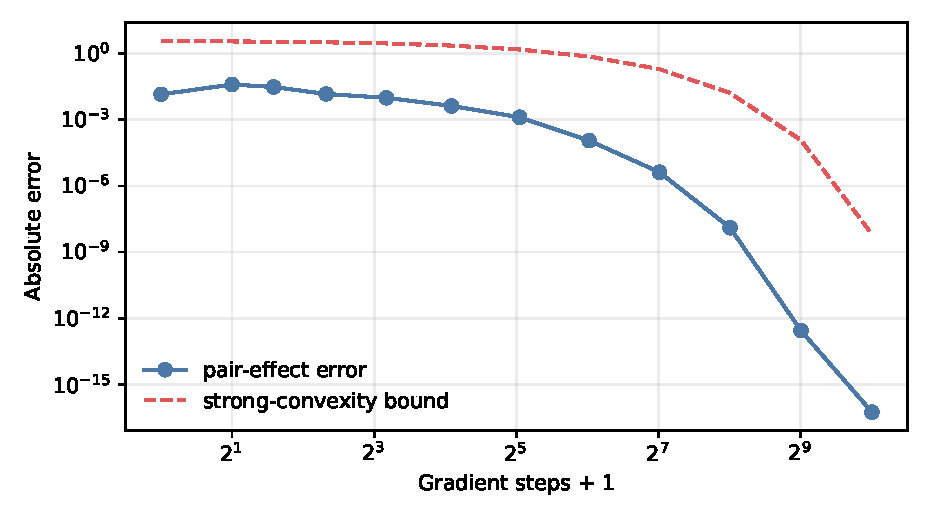
\includegraphics[width=0.72\linewidth]{figures/interaction_finite_response.pdf}
\caption{Convergence of finite-horizon pair effects to the quasistatic effects.
The maximum error decreases from $1.43\times10^{-2}$ at initialization to
$5.55\times10^{-17}$ after 1024 steps and stays below the theoretical bound.}
\label{fig:interaction-finite-response}
\end{figure}

\subsection{Neural response-class audits}

The controlled experiment validates the theorem under global strong
convexity.  We retain the earlier neural audits for a different purpose:
testing whether declared geometric response classes distinguish optimizer
traces in nonconvex training.  A synthetic sanity check first separates fixed
diagonal, time-varying diagonal, momentum, and operator-mixing mechanisms.

\begin{table}[t]
\centering
\caption{Synthetic response-class sanity check.  Raw TGER permits a
step-specific diagonal map; coherent TGER fits one map over the trace.}
\label{tab:followup-synthetic-sanity}
\small
% Generated by experiments/lane_audit/analyze_paper03_followup_runs.py
\begin{tabular}{lrrrr}
\toprule
Mechanism & Mean GER & Raw TGER & Coh. TGER & Gap \\
\midrule
constant diagonal & 1.000 & 1.000 & 1.000 & 0.000 \\
varying diagonal & 1.000 & 1.000 & 0.520 & 0.480 \\
momentum memory & 0.484 & 0.455 & 0.227 & 0.227 \\
decoupled decay & 0.925 & 0.924 & 0.761 & 0.163 \\
operator mixing & 0.785 & 0.785 & 0.494 & 0.291 \\
\bottomrule
\end{tabular}

\end{table}

The long audits record 4096 pre-step gradients and updates for three seeds on
MNIST/Fashion-MNIST and four on CIFAR-10.  Bounded diagonal entries lie in
$[10^{-6},1]$; layer scalar uses one positive scalar per tensor.

\begin{table}[t]
\centering
\caption{Trace-audit seed means.  BDiag uses bounded-diagonal raw TGER under
the raw-gradient convention; +WD changes the visible covector; Layer uses the
layer-scalar family.  Sample standard deviations are retained in the supplied
CSV files.}
\label{tab:rich-convention-summary}
\small
% Generated by experiments/lane_audit/analyze_paper03_rich_runs.py
\begin{tabular}{llrrrr}
\toprule
Dataset & Opt. & Acc. (\%) & BDiag & +WD covec. & Layer \\
\midrule
MNIST & AdamW & 97.6 & 0.274 & 0.256 & 0.086 \\
 & Sophia & 97.5 & 0.187 & 0.278 & 0.029 \\
 & Muon-style & 97.6 & 0.093 & 0.228 & 0.016 \\
 & GNG-Muon & 97.9 & 0.101 & 0.232 & 0.015 \\
\midrule
Fashion-MNIST & AdamW & 88.6 & 0.400 & 0.364 & 0.108 \\
 & Sophia & 88.1 & 0.359 & 0.350 & 0.060 \\
 & Muon-style & 86.9 & 0.137 & 0.241 & 0.016 \\
 & GNG-Muon & 87.3 & 0.137 & 0.241 & 0.015 \\
\midrule
CIFAR-10 & AdamW & 74.6 & 0.367 & 0.338 & 0.088 \\
 & SGD/Nest. & 71.5 & 0.896 & 0.900 & 0.679 \\
 & Lion & 74.2 & 0.400 & 0.336 & 0.188 \\
 & Sophia & 74.7 & 0.345 & 0.335 & 0.035 \\
 & Muon-style & 74.8 & 0.228 & 0.263 & 0.018 \\
 & GNG-Muon & 73.2 & 0.199 & 0.252 & 0.020 \\
\bottomrule
\end{tabular}

\end{table}

\begin{figure}[t]
\centering
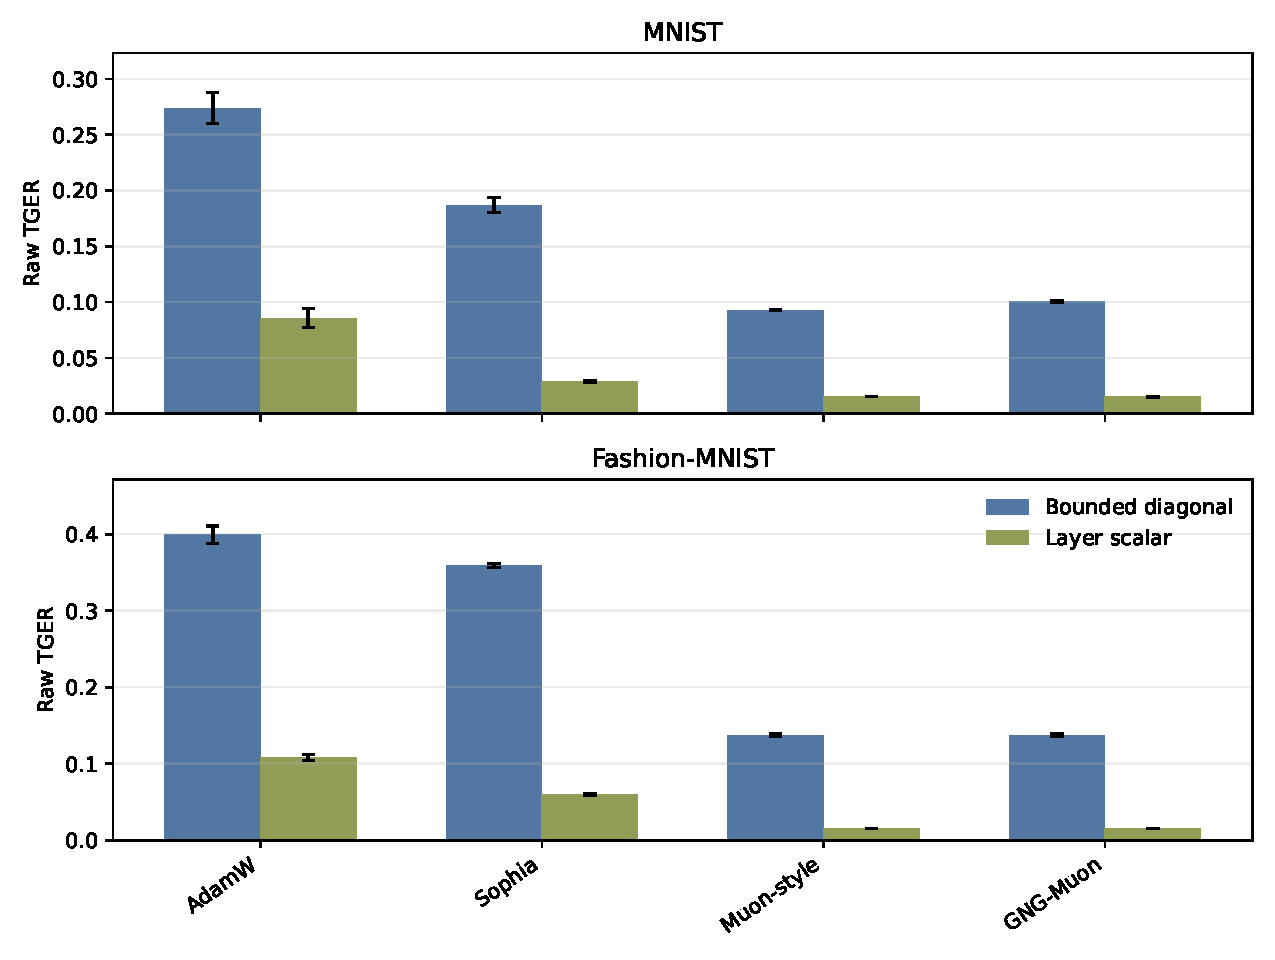
\includegraphics[width=0.72\linewidth]{figures/family_sensitivity_family_comparison.pdf}
\caption{Response-class sensitivity.  Layer scalar is nested inside bounded
diagonal geometry, and the explanation-rate drop varies by optimizer.}
\label{fig:family-sensitivity}
\end{figure}

A follow-up campaign adds channel scalar, an Adafactor-style row, paired
protocol changes, and a tiny-ResNet.  The intervention table reports
ablated-minus-base paired means and sample standard deviations across three
seeds.

\begin{table}[t]
\centering
\caption{Paired protocol interventions.  The SGD contrast jointly removes
momentum and Nesterov structure; the Lion contrast removes the sign operator
and changes update scale at fixed learning rate.}
\label{tab:followup-interventions}
\small
% Generated by experiments/lane_audit/analyze_paper03_followup_runs.py
\begin{tabular}{llrrrr}
\toprule
Intervention & Pair & $\Delta$Acc. & $\Delta$BDiag & $\Delta$Channel & $\Delta$Layer \\
\midrule
weight decay & AdamW $\to$ AdamW/no WD & -0.2$\pm$0.1 & +0.000$\pm$0.001 & -0.000$\pm$0.001 & +0.000$\pm$0.000 \\
momentum/Nesterov & SGD/Nest. $\to$ SGD/no mom. & -18.9$\pm$0.1 & +0.131$\pm$0.009 & +0.218$\pm$0.004 & +0.255$\pm$0.005 \\
sign/scale & Lion $\to$ Lion/no sign & -39.5$\pm$1.9 & +0.191$\pm$0.049 & +0.052$\pm$0.036 & +0.071$\pm$0.036 \\
\bottomrule
\end{tabular}

\end{table}

\begin{table}[t]
\centering
\caption{CIFAR-10 small-ConvNet geometry ladder.  The three columns are nested
response families, not optimizer rankings.}
\label{tab:followup-sector-geometry}
\small
% Generated by experiments/lane_audit/analyze_paper03_followup_runs.py
% small-conv sector run
\begin{tabular}{lrrrr}
\toprule
Opt. & Acc. (\%) & BDiag & Channel & Layer \\
\midrule
AdamW & 61.6 & 0.197 & 0.109 & 0.072 \\
AdamW/no WD & 61.4 & 0.198 & 0.109 & 0.072 \\
SGD/Nest. & 48.7 & 0.750 & 0.510 & 0.471 \\
SGD/no mom. & 29.8 & 0.881 & 0.728 & 0.727 \\
Lion & 50.3 & 0.412 & 0.241 & 0.197 \\
Lion/no sign & 10.8 & 0.603 & 0.293 & 0.268 \\
Sophia & 45.8 & 0.284 & 0.072 & 0.041 \\
Adafactor-style & 46.2 & 0.179 & 0.173 & 0.162 \\
Muon-style & 72.8 & 0.255 & 0.028 & 0.015 \\
GNG-Muon & 72.3 & 0.229 & 0.025 & 0.013 \\
\bottomrule
\end{tabular}

\end{table}

\begin{table}[t]
\centering
\caption{CIFAR-10 tiny-ResNet geometry ladder under the same short-horizon
response audit.}
\label{tab:followup-tinyresnet-geometry}
\small
% Generated by experiments/lane_audit/analyze_paper03_followup_runs.py
% tiny-ResNet run
\begin{tabular}{lrrrr}
\toprule
Opt. & Acc. (\%) & BDiag & Channel & Layer \\
\midrule
AdamW & 58.6 & 0.300 & 0.159 & 0.124 \\
SGD/Nest. & 46.7 & 0.515 & 0.342 & 0.273 \\
Lion & 47.9 & 0.405 & 0.173 & 0.145 \\
Sophia & 39.5 & 0.392 & 0.099 & 0.071 \\
Adafactor-style & 40.7 & 0.217 & 0.216 & 0.210 \\
Muon-style & 61.0 & 0.173 & 0.043 & 0.027 \\
\bottomrule
\end{tabular}

\end{table}

The bundled SGD/Nesterov and Lion sign/scale interventions change both
accuracy and geometric residuals; AdamW weight-decay removal has little effect
over the short trace.  These pairs estimate bundled contrasts and do not
isolate momentum from Nesterov lookahead or sign from update scale.  They also
lack factorial masks and hidden-state measurements.  Accordingly, they support
response-class relevance in nonconvex training, while the digits experiment
provides the direct causal-geometric closure.  The current experiments validate
the P1 reduced-value law and the P3 identification/inference layer; the more
general observable-readout law in \cref{thm:readout-interaction-transfer}
remains an exact analytical prediction for a future nonconvex factorial
campaign.
